\section{Audio and Heartbeat}
The audio and heartbeat system run concurrently with the rest of the program. On an operating system supporting neither processes nor threads that means using interrupts to stop normal execution and perform tasks on the side.\\
\par
When an IRQ triggers an ISR\footnote{Interrupt Service Routine} is called:

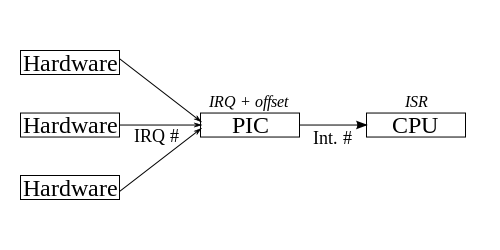
\includegraphics[width=.9\textwidth]{imgs/drawings/irqs/explanation.png}
\par
 Since interrupts keep triggering constantly from various sources, an ISR must make a choice between two ways of operations: Decide it needs a "long" time to run and disable other IRQs via the IMR \footnote{Interrupt Mask Register. Some interrupts like are not maskable}. This way to go introduces the problem of discarding information such as keyboard input or mouse inputs. Or the ISR can decide not to mask other IRQs and return as fast as possible, keeping in mind the routine can be stopped (and never resumed).\\
 \par
 Wolfenstein 3D uses the latter approach and keep things in its ISR very small and short. To this effect everything in the audio and heartbeat system is written in assembly and it avoid "heavy" processing.

\subsection{IRQs and ISRs}
The IRQ and ISR system relies on two chips: The Intel 8254 which is a PIT \footnote{Programmable Interval Timers} and the Intel 8259 which is a PIC \footnote{Programmable Interrupt Controller}. The PIT features a crystal oscillating in square waves. On each edges, it decrements its three counters. When a counter hits zero it generate an IRQ. One of the three counters is connected to the PIC. 
\par
\begin{figure}[H]
\centering
 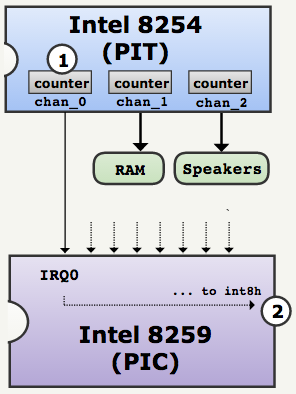
\includegraphics[width=.5\textwidth]{imgs/drawings/heatbeats.pdf}
 \end{figure}
\par

The PIC's IRQ0-IRQ8 is mapped to the Interrupt Vector Offset 8 (resulting in mapping to software interrupts INT08-INT0F).\\

\par
\begin{figure}[H]
\centering
\begin{tabularx}{\textwidth}{ X X  }
  \toprule
  \textbf{IRQ} & \textbf{Type} \\ \bottomrule
0 & System timer \\
1 & Keyboard controller \\
3 & Serial port COM2 \\ 
4 & Serial port COM1 \\
5 & Line print terminal 2 \\
6 & Floppy controller \\
7 & Line print terminal 1 \\
8 & RTC timer \\
12 & Mouse controller \\
13 & Math co-processor \\
14 & ATA channel 1 \\
15 & ATA channel 2  \\
\bottomrule
\end{tabularx}
\caption{Component quality for a game engine.}
\end{figure}
Using these two chips and writing on of its function address into the Interrupt Vector Table, the engine can have one of its method called at a regular time interval, effectively implementing a subsystem running concurrently with everything else.\\



\subsection{PIT and PIC}
The PIT chips runs at 1.193182 MHz. That sounds like an odd arbitrary number which has an uncanny origin. Back in the 1980 when the first IBM PC 5150 was designed, the common oscillator used in television circuitry was running at 14.31818 MHz. In order to reduce part cost, engineers built the PC timer around it, dividing the frequency by 3 for the CPU (that is why the Intel ran at 4.7Mhz), dividing by 4 to 3.57Mhz for the CGA video card. By logically ANDing these signals together a frequency equivalent to the base frequency divided by 12 was created. This frequency is 1.1931816666 MHz. By 1991 the oscillator were much cheaper and it could have been anything but backward compatibility once again dictated otherwise.\\
\par
CODE HERE TO SHOW ISR installation and diff frequencies.



\subsection{Hearbeats}

The only output of the heartbeat system is a 64 bits variable call \cw{TimeCount}:\\
\par
\begin{minipage}{\textwidth}
\lstinputlisting[language=C,morekeywords={longword}]{code/timecount.c}
\end{minipage}
\par
It is updated at a rate of 70 units per seconds (to match VGA which runs at 70Hz). Thse units are called "ticks". Depending on how fast the audio system runs (from 150Hz to 7000Hz) it adjust how much it should increase \cw{TimeCount}.\\
\par
Every system in the engine uses this variable to pace itself. The renderer will not start rendering a frame until at least one tick has passed. The A.I system express action duration in tick units. And so on.\\


\subsection{Music}
Only PC equipped with a FM synthetizer can play music (a.k.a: With an Adlib or a Soundblaster inside). The music system streams data to the sound cards.  Musics in the 90s are not in digitalized format like CD or MP3 nowadays (that would have taken too much storage space and bandwidth). Instead musics are stored on channels (simulating instruments) to which are streamed notes. The format used is close to the notorious MIDI but IMF\footnote{Id Music Format} is proprietary to id software and designed with OPL2 in mind (the raw format is exactly what is sent to the Adlib/Soundblaster synthetiser with no transformations). IMF has hardcoded playback rate and Wolfenstein 3D music run at 700 Hz.\\
\par
Hardware limitations dictated certain aspect of the design of the musics. The FM synthetiser (OPL2) has 9 channels (a.k.a instruments). Yet the composer, Bobby Prince, was asked to use only channel 1 to 8. This little trick wastes a channel on SoundBlaster cards but allows AdLib cards to use channel 0 to play sound simulatenously with the music (the SoundBlaster plays sound differently.).\\









\subsubsection{AdLib/Soundblaster music programming}
\par
Programming the OPL2 ouput was esoteric to say the least. Adlib and Creative did publish SDK but they were very expensive. Documentation was sparse and often cryptic. Two ports, one to select the card register and the other one to read/write data are used:\\
\par
\begin{minipage}{\textwidth}
\lstinputlisting[language=C,morekeywords={longword}]{code/audio_ports.c}
\end{minipage}
\par
When the AdLib first got released in 1986, developers were instructed to send music  to these ports "as fast as possible". At 4.77Mhz a PC was no able to outpace the Adlib. But as CPU got faster issues started to arise. User manual were amended: 


\begin{fancyquotes}
After writing to the register port, you must wait twelve cycles before sending the data; after writing the data, eighty-four cycles must elapse before any other sound card operation may be performed\footnote{http://www.oldskool.org/guides/oldonnew/sound}.
 \bigskip \\
 Alternatively you can issue one IN instruction.
 \bigskip \\
 \end{fancyquotes}
\\
\par
Later, reliable specs were published: "Wait three point three (3.3) microseconds for the address, and twenty-three (23) microseconds for the data."\\
\par










\subsection{Sound effects and Digitized audio}
The engine differenciates between Sound Effects and Digitized Sounds. That is where things become complex:
\par
\begin{figure}[H]
\centering
 \fullimage{audio/audio_settings.png}
 \end{figure}
\par
The audio configuration screen is confusing. Sound effects and Digitized sounds are the same thing: Play sound for a short amount of time but because of the diversity of hardware, sound effects are stored in three formats: Once for PC Speaker, once for Adlib and once for SoundBlaster/Disney Sound Source. The sounds were stored in the same order and separated by format by Muse. The header generated by Muse is seft explanatory.\\

\par
\begin{minipage}{\textwidth}
\lstinputlisting[language=C,morekeywords={longword}]{code/muse_header.c}
\end{minipage}
\par
To transparently store all these sound effects, they are packed in AudioT format, once again an id Software proprietary format. An oditiy: The format can store PC speaker sound, Adlib sound and digitized sounds...but the later is never used. Only PC speaker and Adlib sounds are stored in the \cw{AUDIO.*} files, the digitized sound are in thecw{VMSWAP.*} archive.\\
\note{Question to Johns : Why such a design?} 
\par





\subsubsection{PCM}
Today (2016), digitized sounds have become standard but they were high end in the early 90s. The gave SoundBlaster an edge over Adlib which made them the defactor standard. Sounds are stored in PCM\footnote{Pulse-Code modulation} format where sound is sample at a certain rate, over two channels (left and right) at a certain precision (usually 16 bits values).\\
That encoding it is enough to reconstruct something of high fidelity (as a reference point audio CD uses 44Hz, 16 bits stereo sampling).\\
\par

Wolfenstein 3D sounds are stored in XXX format at XXX rate.



haha: // if the game was paused a LONG time
VGA: 70Hz
audio: Depends on quality, three levels of fidelity.

\par
Stereo system:\\
\par

On a "high-end" stereo SoundBlaster Pro with left and right channel, the sound is more elaborated: The sound source is rotated with the same formula as the raycaster. Using SOH-CAH-TOA. Intensity is hardcoded 0-15:\\
\par
\begin{figure}[H]
\centering
 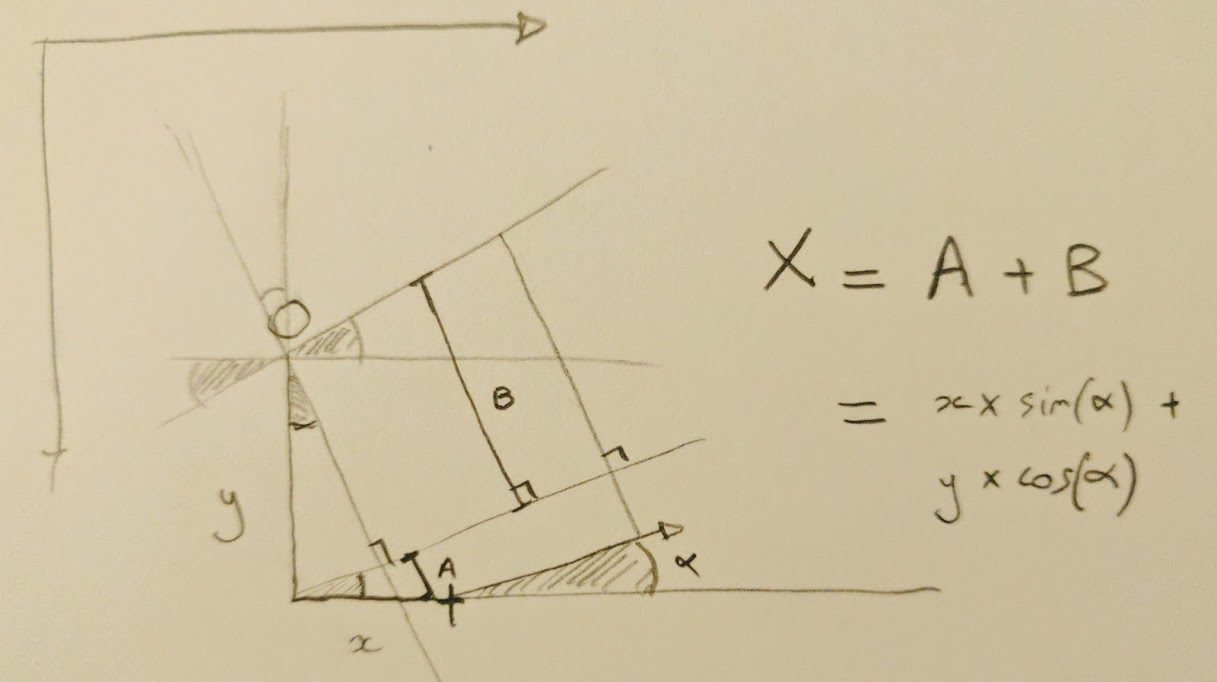
\includegraphics[width=\textwidth]{imgs/drawings/audio_y_rotate.png}
 \end{figure}
 \par
 \begin{figure}[H]
\centering
 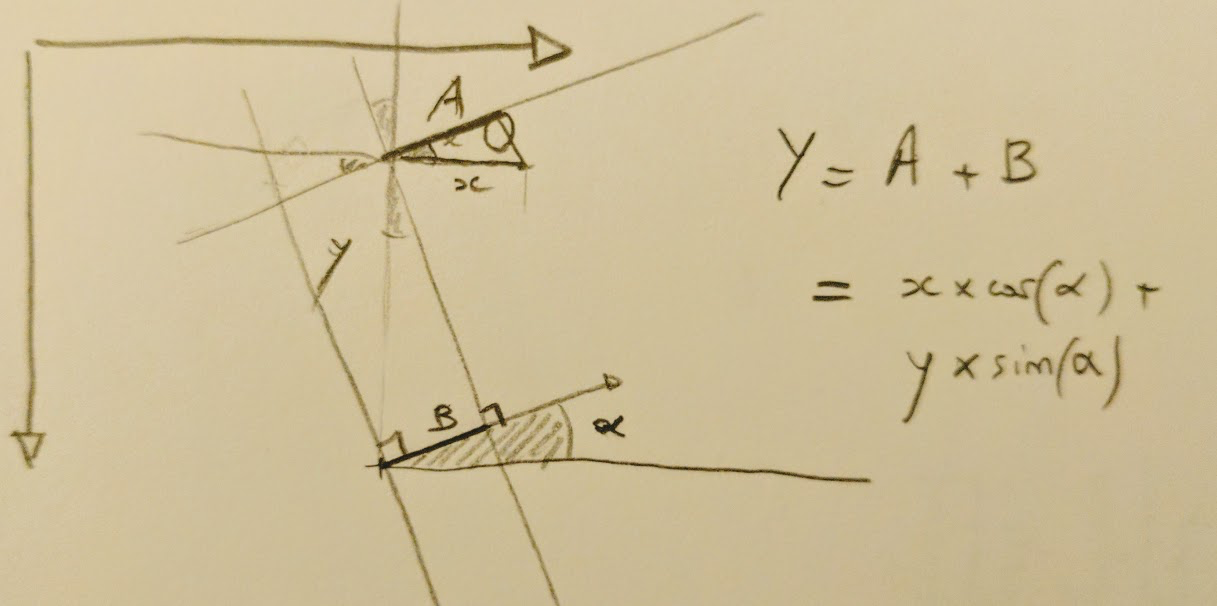
\includegraphics[width=\textwidth]{imgs/drawings/audio_x_rotate.png}
 \end{figure}
\par
In sound part, trivia with a bunch of translations: https://www.gamefaqs.com/pc/564603-wolfenstein-3d/faqs/1824\\
Talk about morse code in episode 3 and 6, echo with romero head in doom2\\
"BLASTER" oldschool parsing.



\subsubsection{Sounds on Adlib}
\subsubsection{Sounds on Disney Sound Source}



\subsubsection{Sound on PC Speaker}
Solving the PC Speaker problem: PWM\\
\par
\begin{verbatim}
"http://www.shikadi.net/moddingwiki/Inverse_Frequency_Sound_format"
\end{verbatim}
The hardware chapter described a problem for sound effects: The default PC speaker can only generate square waves. Pulse Width Modulation, or PWM, is a technique for getting analog results with digital means.




\par
 \begin{fancyquotes}
  The PC speaker is normally meant to reproduce a square wave via only 2 levels of output (the speaker is driven by only two voltage levels, typically 0 V and 5 V). However, by carefully timing a short pulse (i.e. going from one output level to the other and then back to the first), and by relying on the speaker's physical filtering properties (limited frequency response, self-inductance, etc.), the end result corresponds to intermediate sound levels. This effectively allows the speaker to function as a crude 6 bit DAC,[5] thereby enabling approximate playback of PCM audio. This technique is called pulse-width modulation (PWM).
 \end{fancyquotes}
\par
  It gave surprisingly good results such as in Monkey Island music.\footnote{https://www.youtube.com/watch?v=a324ykKV-7Y}

  \par
The programming trick in the PC was to set the timer that drive PC speaker to one-shot mode, and set PC interrupt rate to needed output sample rate. So at every input one sound sample value was read, converted to timer control value, programmed to timer (starting the pulse). This trick allowed around 6 bits sample resolution / dynamics (or even slightly more with some tricks). When the sample rate was high enough, you can’t hear the high frequency noise on the signal.\\
TODO: Drawing of PWM
\par
Mode 1 - Hardware Re-triggerable One-shot\\
Mode 2 - Rate Generator\\
Mode 3 - Square Wave Generator\\
Mode 4 - Software Triggered Strobe\\
Mode 5 - Hardware Triggered Strobe\\
\par
\begin{figure}[H]
\centering
 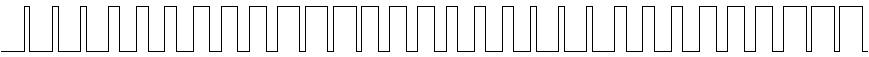
\includegraphics[width=\textwidth]{imgs/drawings/pwm/sinuois.png}
 \end{figure}
\par

\par
\begin{figure}[H]
\centering
 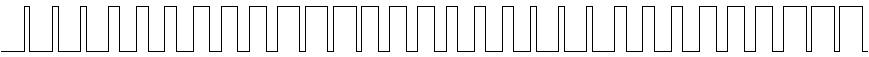
\includegraphics[width=\textwidth]{imgs/drawings/pwm/pwm_approximation.png}
 \end{figure}
\par


The audio and heatbeat system are started. This is done by reprogramming 8254-PIT and 8259-PIC timers to install an ISR\footnote{DOS Interrupt Service Routine}:\\

frequency = 1193181 / (value * 60)\\
Inverse Frequency Sound format\\
\par
\begin{figure}[H]
\centering
 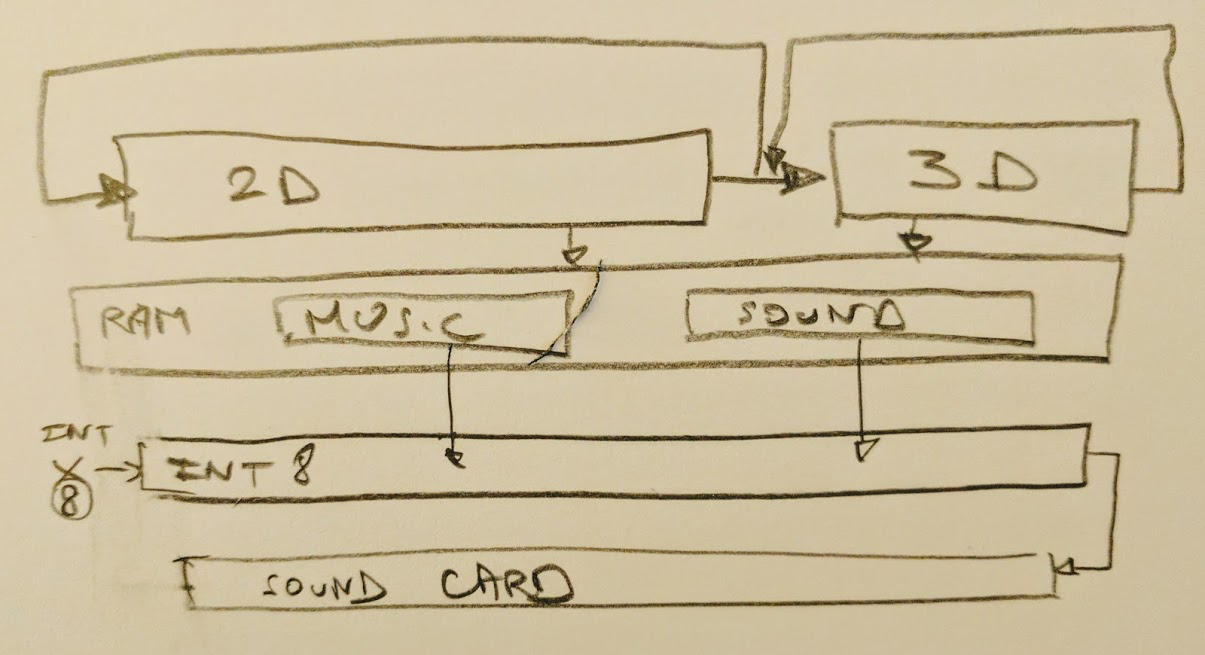
\includegraphics[width=\textwidth]{imgs/drawings/three_blocks.png}
 \end{figure}

Different things could happen depending on the hardware available:
\begin{itemize}
\item With the default PC speaker or with , the isr is set on slow: 140Hz
\item With an adlib or Disney Sound source, the isr is set on fast: 700Hz
\item With Sound Blaster, the isr is set on extreme: 7000Hz
\end{itemize}
Every time the ISR triggers, it takes care of feeding music and audio to the sound chip and also updates TimeCount variable, the heat of the whole system, at 70Hz (like VGA refresh rate).\\
\par
Because the engine uses triple buffering, it is completely decoupled from the VGA refresg rate (70Hz). Yet it needs something not only to pace itself (not render too fast) and to keep track of wall time (so the player is presented with a linear game time progression). This is where the sound system performs two tasks. Not only the XXX chips triggers at a regular interval, it also updates a global variable (\cw{TimeCount}) at 70Hz. This variable is used in the renderer to make sure at least 1/70th of a second has passed before rendering something again but also to pace actor thinking (so player movement is proportionnal to frame rate and actor also think proportionnaly).\\
\cw{CalcTics} maintains \cw{ticks} variable: The amount of walltime since last frame. An action takes a certain number of ticks.\\
\par
It works but there is a major flaw with this technique: The engine is non-deterministic. Recording and replaying a demo, even on the same machine cannot work.\\\par
haha joke about LONG time.\\
\bu{Trivia :} When playing a recording, the engine bypasses the timer and hardcoded tics: (tics = DEMOTICS;). The demo was likely recorded at 15fps which is consistent with what a 386DX33 would have produced

\subsubsection{TODO}
Talk about DMA requests from Sound Blaster.\\
\par
TAlk about soud blaster parsing of options.\\
\begin{minipage}{\textwidth}
\lstinputlisting[language=C]{code/soundblasterconf.c}
\end{minipage}


PC Speaker to play Digitized sounds ? How  ?\footnote{You can hear the difference here: https://www.youtube.com/watch?v=1BtlsjJRnFU}\\





















